%!TEX root = ../../thesis.tex
%*******************************************************************************
%****************************** Design Chapter *********************************
%*******************************************************************************

\chapter{Solution Design}
\label{chap:design}

\ifpdf
    \graphicspath{{Chapters/Design/Figs/}{Chapters/Design/Figs/}{Chapters/Design/Figs/}}
\else
    \graphicspath{{Chapters/Design/Figs/}{Chapters/Design/Figs/}}
\fi
In the previous chapter, we defined various terminologies and concepts that we are using for our thesis.
Based on that, in this chapter, we derive some design concepts required for our \ac{dsr}.
Therefore, we explore the \ac{dr} (see section \ref{design:section:designReqs}), \ac{dp} (see section \ref{design:section:designprinciple}), and an overall solution design (see section \ref{design:section:solutiondesign} which gives an incite of the creation of our solution approach) to guide the result of our software tool.
Design is a critical aspect of \ac{se}, providing the blueprint for implementing functional and non-functional requirements. 
The design phase is crucial in ensuring that software systems are developed efficiently, effectively, and with high quality. 
We develop our design approach based on the principles of \ac{dsr}. 
Through this exploration, we will provide an in-depth understanding of the design process, highlighting the key factors that must be considered to create effective software solutions.

%********************************** % Design Requirements **************************************
\section{Design Requirements (DRs)}
\label{design:section:designReqs}
\ac{dr}s in \ac{dsr} are typically defined as a set of constraints and specifications that must be met by the design artifact to be considered a successful solution. 
These requirements can be functional, such as the specific features or capabilities that the design/tool must have, or non-functional, such as performance, usability, or scalability.
In our findings of the \ac{dr}s, we focus more on the functional requirements and ignore the non-functional.
To derive a solution, we define some \ac{dr}s with the help of the literature review\footnote{It was a non-systematic literature review by reading research papers and looking at some renowned UI prototyping tools. The related literature is available in Appendix \ref{appendix:two:definations}} and comparison of some tools.
In this context, each \ac{dr} refers to a generalized requirement that can be standardized and applied to future software applications.
We covered a wide range of topics including \textit{\ac{ui} Prototyping}, \textit{Low-Code/No-Code development}, \textit{Model-Based Software Engineering}, \textit{Continuous Experimentation}, \textit{Task-Based Usability Testing}, and the \textit{LEAN development process}.
The following section presents \textit{nine \ac{dr}s} that explains the requirements for the approach \textit{(solution approach)} and their corresponding references in literature and tools.
% \paragraph*{Systematic literature reviews:} 
% Systematic literature reviews establish a solid basis for knowledge creation. 
% They help create theories and identify areas that require more research.
% By identifying existing literature and highlighting areas to explore, they also assist in the understanding of the problem space in DSR.
% Therefore, a comprehensive DSR project must include systematic literature reviews \cite{misc:dsr:webster}.
% \paragraph*{Interviews:}
% Interviews are regarded as empirical research to obtain primarily qualitative insights from individuals, such as specialists in a particular subject. 
% Suppose the interviewers are a part of the problem's stakeholder group.
% In that case, they may be utilized to establish requirements (or meta requirements) for the solution space that have a solid foundation for the problem space.
% For example, artifacts can be designed based on design principles (DPs) generated from interviews.
% Furthermore, the interviews can also be used to improve and evaluate the designed artifacts \cite{misc:dsr:mayring}. 
% \paragraph*{Other Methods:}
% Design requirements can also be generated using other methods or combinations of methods.
% Other methods include simulations, experiments, case studies, ethnography, and the grounded theory approach \cite{misc:dsr:nickerson, misc:dsr:varshney}. \\\\

\paragraph{\ac{dr}1: Heterogeneous Users} states that \textit{the approach should support diverse users with different needs, goals, and capabilities and integrate internal and external users.} 
It is supported by literature indicating that different users may have different needs, preferences, and levels of technical expertise \cite{misc:lean:steve}.
By including a diverse group of users, you can get a broader range of feedback and insights into how the software performs for different users \cite{article:prototyping:weichbroth}, and reduces the biases among developers \cite{misc:lean:burmeister}.
In this context, the users can be from internal sources, such as employees, or external sources, like Amazon Mechanical Turk\footnote{Amazon Mechanical Turk: \url{https://www.mturk.com/}} for using the software.

\paragraph{\ac{dr}2: Iterative Design} states that \textit{the approach should be designed in an iterative, incremental method to help identify and address any technical issues or design flaws early in the development process for achieving the goals.} 
It is supported by literature indicating that the iterative approach involves the idea of breaking down development into small, incremental cycles of work rather than trying to deliver a complete product all at once \cite{misc:lean:tutorial}.
The key benefit of an iterative approach is that it allows the development team to get feedback from users and stakeholders early in the development process and to make adjustments \cite{article:experiments:lindgren} to the product as needed.

\paragraph{\ac{dr}3: Easy Development} states that \textit{the approach should be easy to develop and operatable by non-technical individuals with drag-and-drop interfaces and pre-built components to create applications without extensive programming knowledge.} 
It is supported by literature indicating that a tool should have a UI that helps non-technical individuals to build software without including the developers. 
It can be achieved if the tool provides drag-and-drop interfaces \cite{article:nocode:miller}, reusable pre-built components \cite{article:prototyping:lowcode} (e.g., buttons, textbox, and other \ac{ui} components, data models for data transfer between components) and a logical flow (E.g., \textit{Screen1} is followed by \textit{Screen2} and so on.). 
In many tools like \texttt{Figma\footnote{Figma Prototyping tool: \url{https://www.figma.com/}}}, \texttt{Invision\footnote{Invision: \url{https://www.invisionapp.com/}}}, and \texttt{Axure\footnote{Axure Rapid Prototyping: \url{https://www.axure.com/}}}, we saw these features.

\paragraph{\ac{dr}4: Integrate Data Models} states that \textit{the approach should be designed to make it easier to integrate data models by providing pre-built connectors and APIs that can be used to connect to various data sources.} 
It is supported by literature indicating that by using the tool, citizen developers can easily access and integrate data models from multiple sources, including databases, APIs, and external systems \cite{paper:lowcode:khorram}, without having to write complex code or build custom integrations from scratch \cite{article:lowcode:modeldriven}.
It accelerates the development process, reduces the risk of errors \cite{misc:lowcode:platforms}, and improves the software tool's overall quality.
In many tools like \texttt{Figma}, \texttt{Invision}, and \texttt{Axure}, we saw the use of data models\footnote{These tools either have their own implementation or depend on some third-party data model tool.}.

% \paragraph{\ac{dr}5: Engage Stakeholders} states that \textit{Various stakeholders (e.g., designers, product managers, developers, etc.) must contribute to the quick development of the product.}
% It is supported by literature indicating that involving different project stakeholders and providing them with the necessary communication tools helps exchange and codify knowledge \cite{article:prototyping:weichbroth}. 
% This makes sure that the stakeholders' perspectives, requirements \cite{misc:prorotypes:lauff}, and their input helps shape the product's design.

% \paragraph{\ac{dr}5: Diverse Re-usable components} states that \textit{Collaboration between different team members and usage of the reusable components of various disciplines should make the tool easy for anyone to use on any platform and share their work quickly.} 
% It is supported by literature indicating developers' ability to create more consistent, user-friendly prototypes that adhere to the re-usable components' established style and principles \cite{paper:prototyping:luqi} and help improve the overall design process and product development \cite{article:prototyping:hoffnagle}.
% In many tools, we saw the use of many reusable components like buttons, textbox, and other \ac{ui} components, data models for data transfer between components, and some guidelines to promote accessibility and usability of the tools.

\paragraph{\ac{dr}5: Construct User Scenarios} states that \textit{the approach should be used to observe and record how users interact with a software tool by completing a series of tasks to evaluate the tool's ease of use.} 
It is supported by literature indicating that testing of the \ac{gui} of a software application is done using functional and usability tests \cite{misc:usability:tasks}. 
This helps the developers to identify any usability issues \cite{article:tbup:kari} and improve them continuously \cite{article:prototyping:gould}.
And this helps in the identification and preliminary validation of user requirements in the early stages of development \cite{article:prototyping:weichbroth}. 

% \paragraph{\ac{dr}7: Improved Accessibility} states that \textit{The tool should be a web-based application making it accessible and independent of any software, platforms (e.g., Macbooks, Windows \ac{pc}s, Linux machines, Chromebooks) and have an auto-save feature to store the work on Cloud.}
% It is supported by literature indicating that Web-based tools have several advantages \cite{misc:cloud} over traditional application-based tools.
% In many tools like \texttt{Figma}, \texttt{Invision}, and \texttt{Axure}, we saw features\footnote{Some more features: \url{https://redrocksoftware.com.au/10-benefits-of-web-based-applications-systems/}} like \texttt{Accessibility} i.e., can be accessed from any device with an internet connection, \texttt{Collaboration} i.e., have built-in collaboration features, making it easy for team members to work on the same prototype simultaneously, \texttt{Updates} i.e., automatically updated.

% \textbf{DR9: Get user feedback} \textit{} Having users perform specific tasks and observe how they interact with the application helps improve the usability of the software applications. So, we can use task-based usability testing for achieving this. 
\paragraph{\ac{dr}6: Collect Feedback} states that \textit{the approach should gather various user feedbacks (such as user behavior patterns, click rates or open-ended questions) from the split tests.}
It is supported by literature indicating that feedback can be collected while observing the participants performing the tasks \cite{misc:qualitative:qualitative}, like asking open-ended questions about their overall experience.
At the same time, it should automatically record any feedback that participants give and analyze it while looking for some pattern in the data \cite{article:qqa:young}.

\paragraph{\ac{dr}7: Aggregated Feedback} states that \textit{the approach should gather user feedback and aggregate them to make improvements to the application.} 
It is supported by literature indicating that \texttt{Qualitative analysis} gathers an in-depth understanding of underlying reasons, opinions, and motivations \cite{misc:dsr:mayring}.
Whereas \texttt{Quantitative analysis} measures and understands numerical data and helps identify patterns and trends \cite{article:qqa:young}.
An aggregation of the qualitative and quantitative analysis can provide a more complete picture of a situation and can be used to validate or disprove findings from one type of analysis \cite{article:qq:helena}.

\paragraph{\ac{dr}8: Visualize Feedback} states that \textit{the approach should provide visual representations of data visualization such that users can better understand and interpret the presented data and gain insights that might only be apparent through raw data.} 
It is supported by literature indicating that visualization helps in prototyping by allowing designers and stakeholders to see and understand the design in a way that is easy to understand \cite{article:comparative:prototypes}.
It also allows designers to identify usability issues \cite{article:prototyping:gould} early in the design process to make the end product user-friendly and easy to use.
In tools, various methods, like creating \textit{Graphs}, \textit{Charts}, \textit{Plots}, etc. are used for visualization.

% \paragraph{\ac{dr}10 Quick delivery} states that \textit{A software product should be easily deliverable, reducing the complexity and deployment time and increasing the product's usability.} 
% It is supported by literature indicating that when software is easy to build, development teams can be more productive and efficient, leading to lower development costs \cite{misc:lowcode:platforms} and can be quickly delivered. 
% It's also easy for different development team members to understand and work on the code, thereby improving collaboration \cite{misc:prorotypes:lauff} and generating high-quality code.
% Adding new features, scaling up, and making changes, as needed, make the tool more accessible and helpful \cite{article:prototyping:lowcode} to ensure that the product is developed and deployed with minimum effort \cite{article:prototyping:lowcode}.

\paragraph*{\ac{dr}9: Classified UI variants} states that \textit{the approach should create multiple variants or versions of a user interface, each with distinct UI elements or features, to evaluate their impact on user engagement and performance.}
It is supported by literature indicating that a product can be tested against different design solutions and variations \cite{article:CE:fitzgerald} to see which variant performs the best in terms of usability, aesthetics, and other characteristics \cite{article:controlled:experiements}. 
At the same time, continuously improve \cite{article:CE:ros} the product based on the feedback of the best-fit variant.

% \paragraph*{\ac{dr}10: Provide feedback assistance} states that \textit{A Software product should help the citizen developers with the analysis by guiding them on what questions should be asked to the participants.}
% It is supported by literature indicating that there are many ways of creating qualitative analysis questions \cite{misc:dsr:mayring} confusing the citizen developers on deciding the correct approach \cite{misc:qualitative:qualitative}.
% Therefore, there should be a recommendation system for suggesting the relevant questions called post-task questionnaires.
% Some examples\footnote{Examples post-task questionnaires: \url{https://uxpsychology.substack.com/p/standardized-usability-questionnaires-ccb}} are ASQ\footnote{ASQ (After Scenario Questions): \url{https://ehealth.uvic.ca/resources/tools/UsabilityBenchmarking/05a-2011.02.15-ASQ_and_PSSUQ_Questionnaires-no_supplements-v3.0.pdf}} (After Scenario Questionnaire) which consists of 3 questions, SMEQ (Subjective Mental Effort Questionnaire) which is composed of 1 question, etc. 

\clearpage
%********************************** % Design Principles **************************************
\section{Design Principles (DPs)}
\label{design:section:designprinciple}
\ac{dp}s are guidelines or rules used to guide the design process in \ac{dsr} \cite{misc:dsr:henver}. 
They provide a framework for making design decisions \cite{paper:designprinciple:gregor} and help to ensure that the final solution meets the goals and objectives of the research. 
This section codifies our knowledge during the design study and derives \ac{dp}s from abstract \ac{dr}s in the iteration cycle of the \ac{dsr}.
The following shows the \textit{nine \ac{dp}s} for \textit{our solution approach} that is built on the foundation of the mapped \ac{dr}s (see figure \ref{fig:design:table-drs-dps}). 
\begin{figure}[htbp!]
  \centering    
  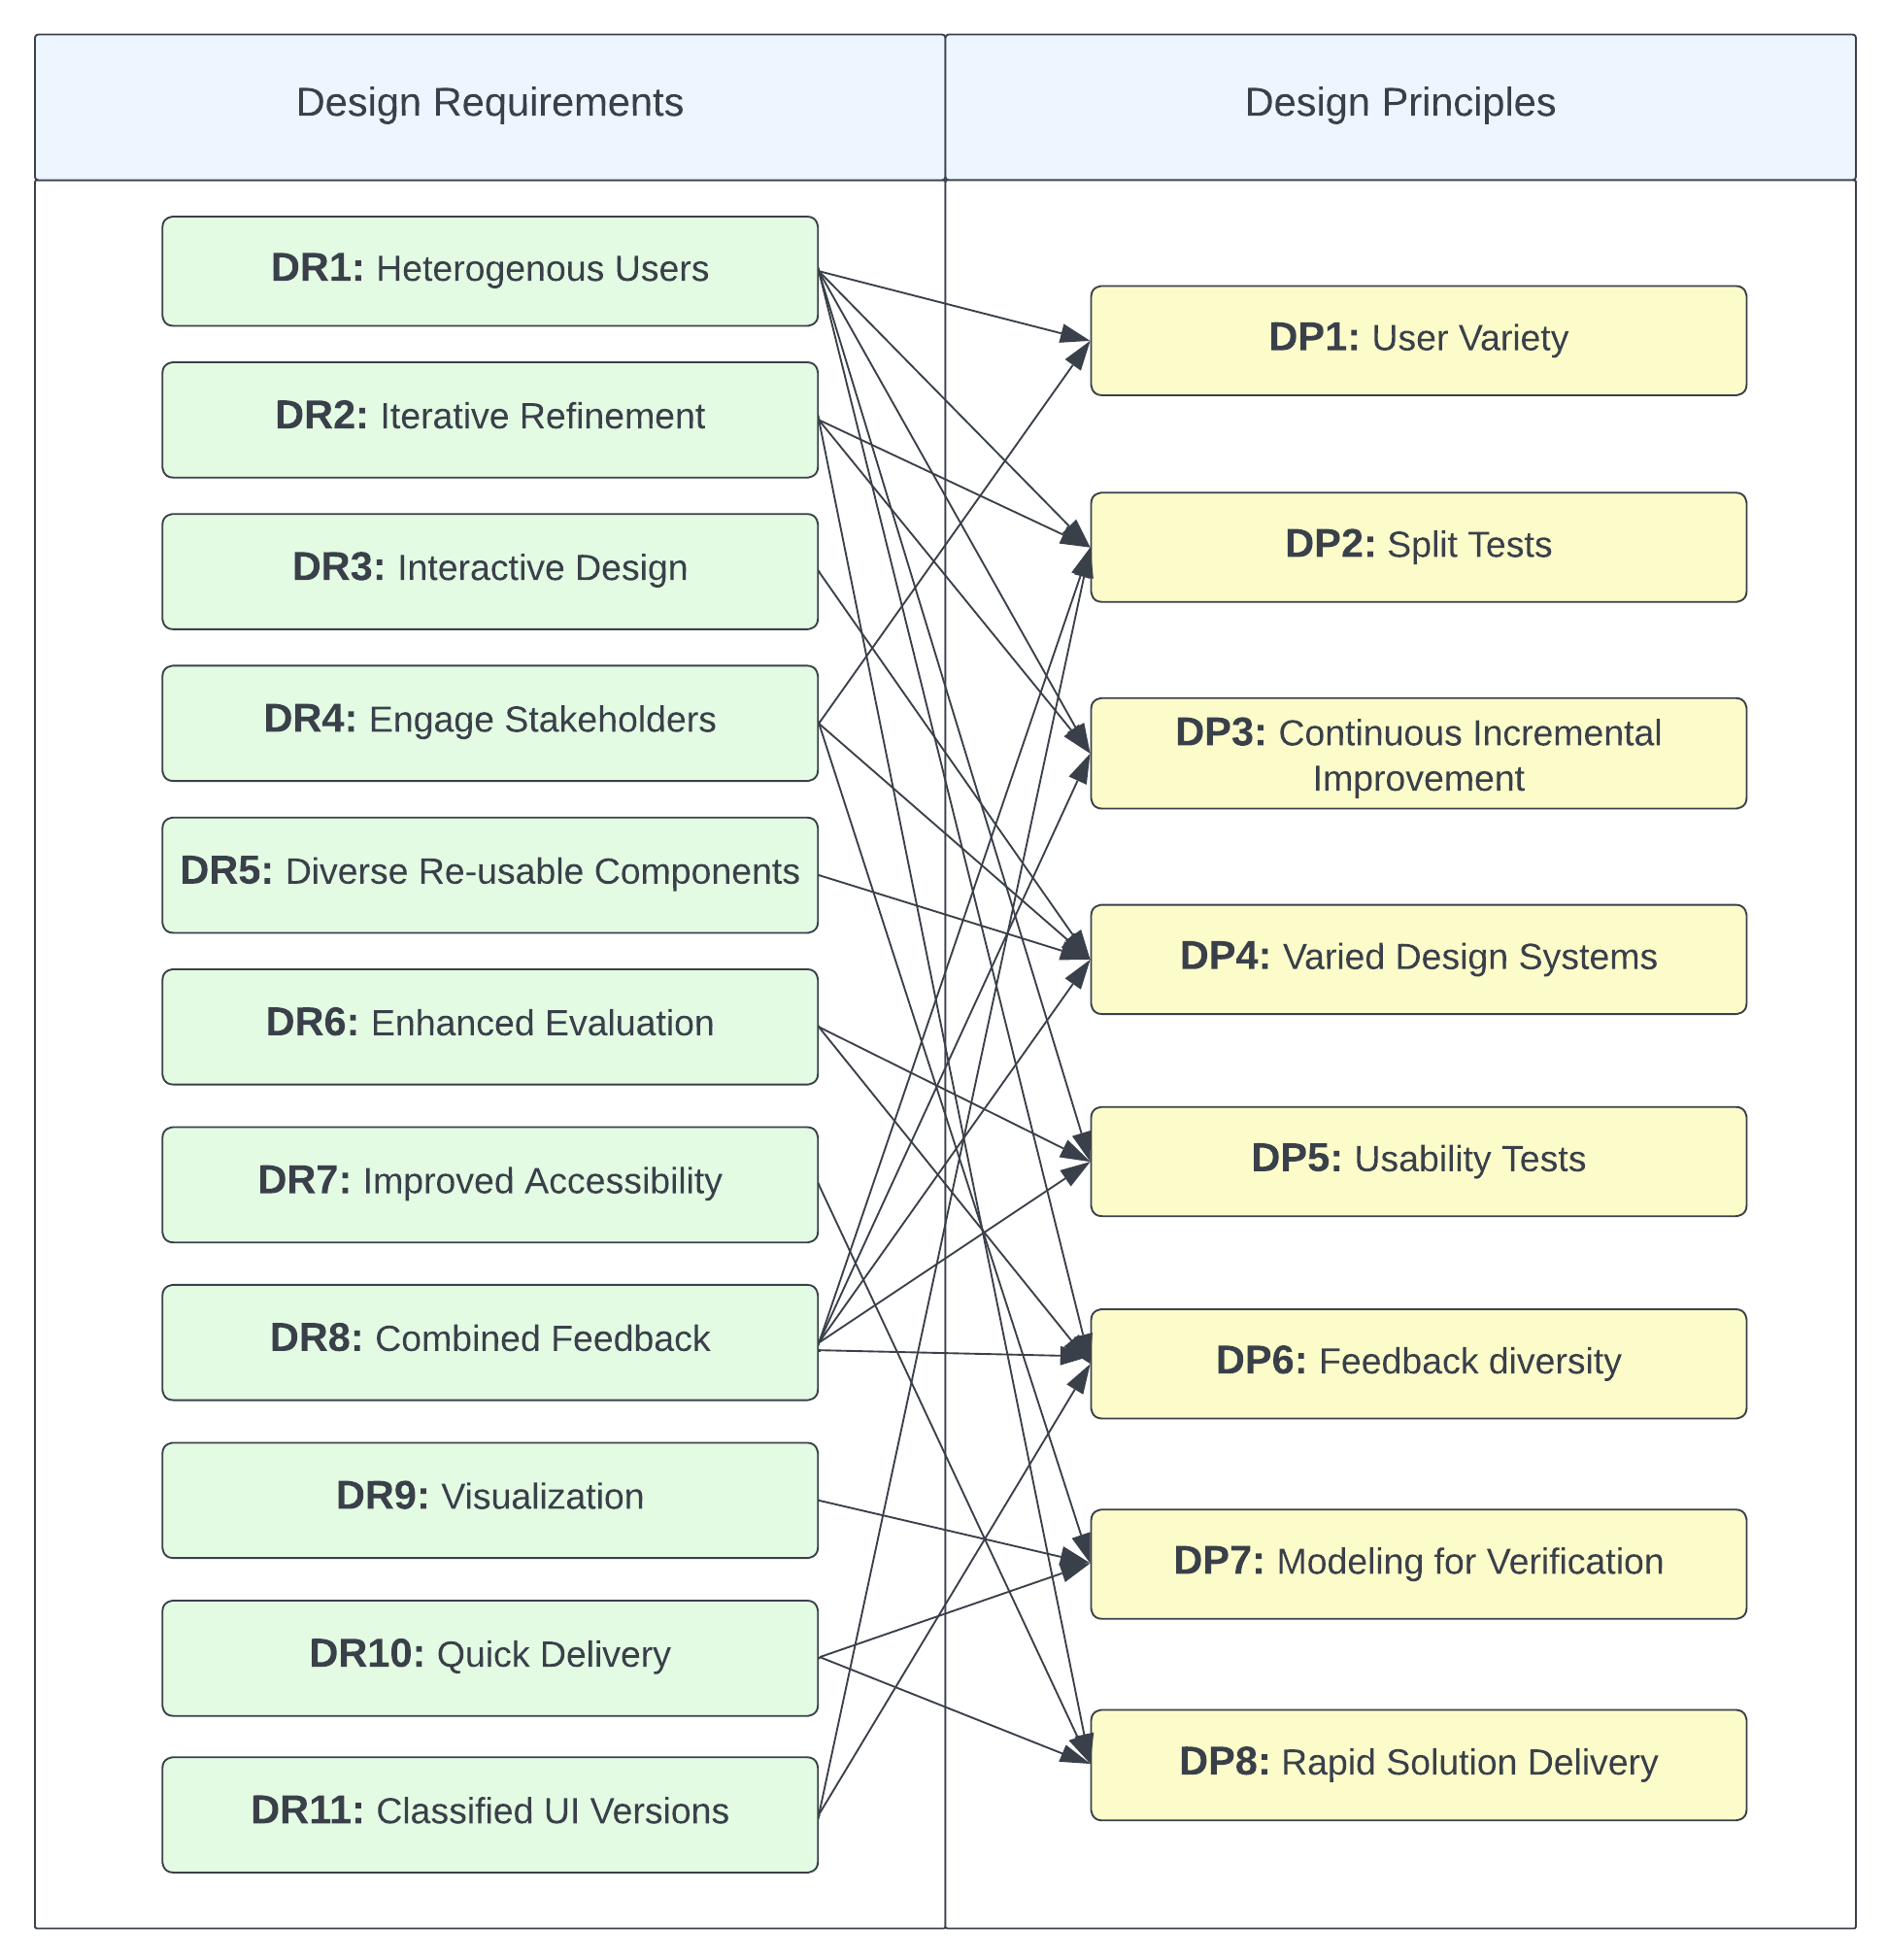
\includegraphics[width=0.85\textwidth]{Table-drs-dps.png}
  \caption[A map between \ac{dr}s and \ac{dp}s]{A map between \ac{dr}s and \ac{dp}s}
  \label{fig:design:table-drs-dps}
\end{figure}

\paragraph{\ac{dp}1: User Variety:} \textit{The solution approach is required to have provisions that enable the integration of diverse types of users, both internal and external (e.g., tool users and crowd workers), so that developers can engage with various users during the evaluation process.}

Developers have many unclear generalities early in the product development process \cite{misc:lean:steve} that they can clarify by testing the underlying assumptions using different types of users (i.e., \textit{DR1: Heterogenous Users}), and involving various product stakeholders using an iterative design for continuous improvement (i.e., \textit{DR2: Iterative Design}).
This helps to gather the user requirements smoothly, thus improving the product's usability.

\paragraph{\ac{dp}2: Split Tests:} \textit{The solution approach is required to have provisions to create different versions of UI prototypes and conduct A/B testing to compare the performance of each version so that developers can make data-driven decisions about which UI design works best for their users.}

Split Tests (also known as A/B Testing) are performed on a randomly divided sample group of different users (i.e., \textit{DR1: Heterogenous Users}) by exposing each group to the \ac{ui} of different versions (i.e., \textit{DR9: Classified UI variants}) to find out the feature that is most usable and functional for the users.
The results of the test are then used to determine which version is more effective by aggregating the feedback (i.e., \textit{DR7: Aggregated Feedback}) from the user groups and finally optimizing the whole product.

\paragraph{\ac{dp}3: Continuous Design:} \textit{The solution approach is required to have provisions to design the tool into small, incremental phases in the software development process so that developers can improve software delivery and make product changes and improvements based on customer feedback.}

Using a continuous incremental approach, we can continuously improve software products by delivering value to customers as quickly as possible \cite{misc:lean:toyota}, constantly refining and improving the product \cite{misc:lean:planning}, and delivering the product as soon as possible.
Here, the iterative design should be used (i.e, \textit{DR2: Iterative Design}) to get continuous feedback from a variety of users (i.e., \textit{DR1: Heterogenous Users}).
The feedback which is collected should be a combination (i.e., \textit{DR7: Aggregate Feedback}) of various feedback helping significantly improve the application.

\paragraph{\ac{dp}4: Pre-Designed Interactive UI Elements:} \textit{The solution approach is required to have provisions containing a library of pre-designed UI elements (such as buttons, menus, and forms) and interactive components (such as textbox, checkbox, and data models) that can be easily customized and used in the prototype so that developers can demonstrate how the \ac{ui} will function.}

A \ac{ui} Prototyping tool is helpful when different interactive (i.e., \textit{DR3: Easy Development}) re-usable components are used as a drag-and-drop element while creating the prototypes by adding various data models (i.e., \textit{DR4: Integrate Data Models}). 
It helps to get more feedback from the users or the participants, improving the product's usability and functionality.
% In many tools, we saw the use of many \ac{desy} like \texttt{Design System Components} (e.g., buttons, forms etc.), \texttt{Design System Patterns} (e.g., patterns for communication and data transfer between components), \texttt{Accessibility standards} (e.g., some guidelines to promote accessibility).

\paragraph{\ac{dp}5: User tasks Refinement:} \textit{The solution approach is required to have provisions to create tasks that simulate real-world scenarios and workflows, with clear instructions and defined success criteria, and assign randomly to participants so that developers can collect and improve the UI prototype with the help of data.}

We can improve the usability of software by observing different users (i.e., \textit{DR1: Heterogenous Users}) as they interact with the product and measuring how well they can accomplish specific tasks or goals (i.e., \textit{DR5: Construct User Scenarios}).
Moreover, the users can provide valuable insights into how easy or difficult it is to use the product and help identify areas where developers could improve the UI or design aggregating user feedback (i.e., \textit{DR7: Aggregated Feedback}).

\paragraph{\ac{dp}6: Qualitative Analysis:} \textit{The solution approach is required to have provisions for collecting and analyzing qualitative feedback from participants, such as comments, feedback forms, or open-ended questions so that developers can gain insights into the user experience and identify areas for improvement.}

We can conduct qualitative analysis systematically for examining non-numerical data to uncover patterns, themes, and insights from different users (i.e., \textit{DR1: Heterogenous Users}). 
It can be achieved through various methods (i.e., \textit{DR6: Collect Feedback}) such as content analysis, grounded theory, or discourse analysis, which involve careful coding, categorization, and interpretation of the data.

\paragraph{\ac{dp}7: Quantitative Analysis:} \textit{The solution approach is required to have provisions for quantitative analysis features so that developers can analyze and visualize data from A/B testing and other analytics, such as user behavior patterns, click heatmaps, and conversion rates and improve the \ac{ui} prototype.}

We can conduct quantitative analysis systematically to test hypotheses, measure relationships between variables, and make statistical inferences about populations based on representative samples from different users (i.e., \textit{DR1: Heterogenous Users}).
It can be achieved by assigning tasks to various users in the study (i.e., \textit{DR5: Construct User Scenarios}) and collecting theier feedbacks (i.e., \textit{DR6: Collect Feedback}).

\paragraph{\ac{dp}8: Diversity in Analytics:} \textit{The solution approach is required to have provisions for different analytics and metrics (qualitative and quantitative) so that developers can track the performance and behavior of the different \ac{ui} prototypes variants being tested.}

Performing various tests (e.g., usability testing) with diverse users (i.e., \textit{DR1: Heterogenous Users}) ensures that the software is accessible and easy to use for different groups of people with an accurate evaluation of the task provided to the users (i.e., \textit{DR5: Construct User Scenarios}).
Moreover, diversity in software development feedback mechanisms (i.e., \textit{DR6: Collect Feedback}), received by testing different UI versions (i.e., \textit{DR9: Classified UI variants}), helps ensure the software is inclusive and accessible.

\paragraph{\ac{dp}9: Modeling:} \textit{The solution approach is required to have provisions for models that can be used to simulate the behavior of the UI prototype so that developers can test its functionality and identify potential issues before the actual software is developed.}

Modeling increases transparency among various stakeholders, increasing their contribution to the product due to their excellent visualization capability (i.e., \textit{DR8: Visualize Feedback}).
Furthermore, modeling tools can automatically generate code or other documentation from the models, which can help reduce errors, improve efficiency, and decrease development time iteratively (i.e., \textit{DR2: Iterative Design}).

% \paragraph{\ac{dp}10: Feedback assistance:} \textit{By providing guidelines on what type of questions (rating based or open-ended) to ask of the participants, the software product should aid citizen developers with qualitative analysis.}

% We can provide a feedback assistance system (i.e., \textit{\ac{dr}12: Assistance for Feedback}) for qualitative analysis helping the citizen developers formulate a qualitative questionnaire. 
% These questions can be asked to the participants either during the tasks or after the completion of the task (i.e., \textit{\ac{dr}6: Enhanced Evaluation}) as a post-survey questionnaire. 
% Thus, having a predefined qualitative questionnaire helps to automate the feedback mechanism (i.e., \textit{\ac{dr}8: Combined Feedback}).

\clearpage
%********************************** % Solution Concept **************************************
\section{Overall Solution Design}
\label{design:section:solutiondesign}
As shown in figure \ref{fig:design:lean}, we conceptualize the solution design from our codified \ac{dp}s.
The software platform consists of two types of roles consisting of the Stakeholders for creating the Prototyping tool (Admin users like, \textit{Product Owners}, the \textit{Designers}) and the \textit{Users or Participants} for testing the tool.
In this section, we arrange our \ac{dp}s using a LEAN development approach\footnote{Adopted from LEAN process development: \url{https://www.lean.org/explore-lean/product-process-development/}}, a cycle consisting of \textit{Build}, \textit{Measure}, \textit{Learn} phases.

\begin{figure}[htbp!]
  \centering    
  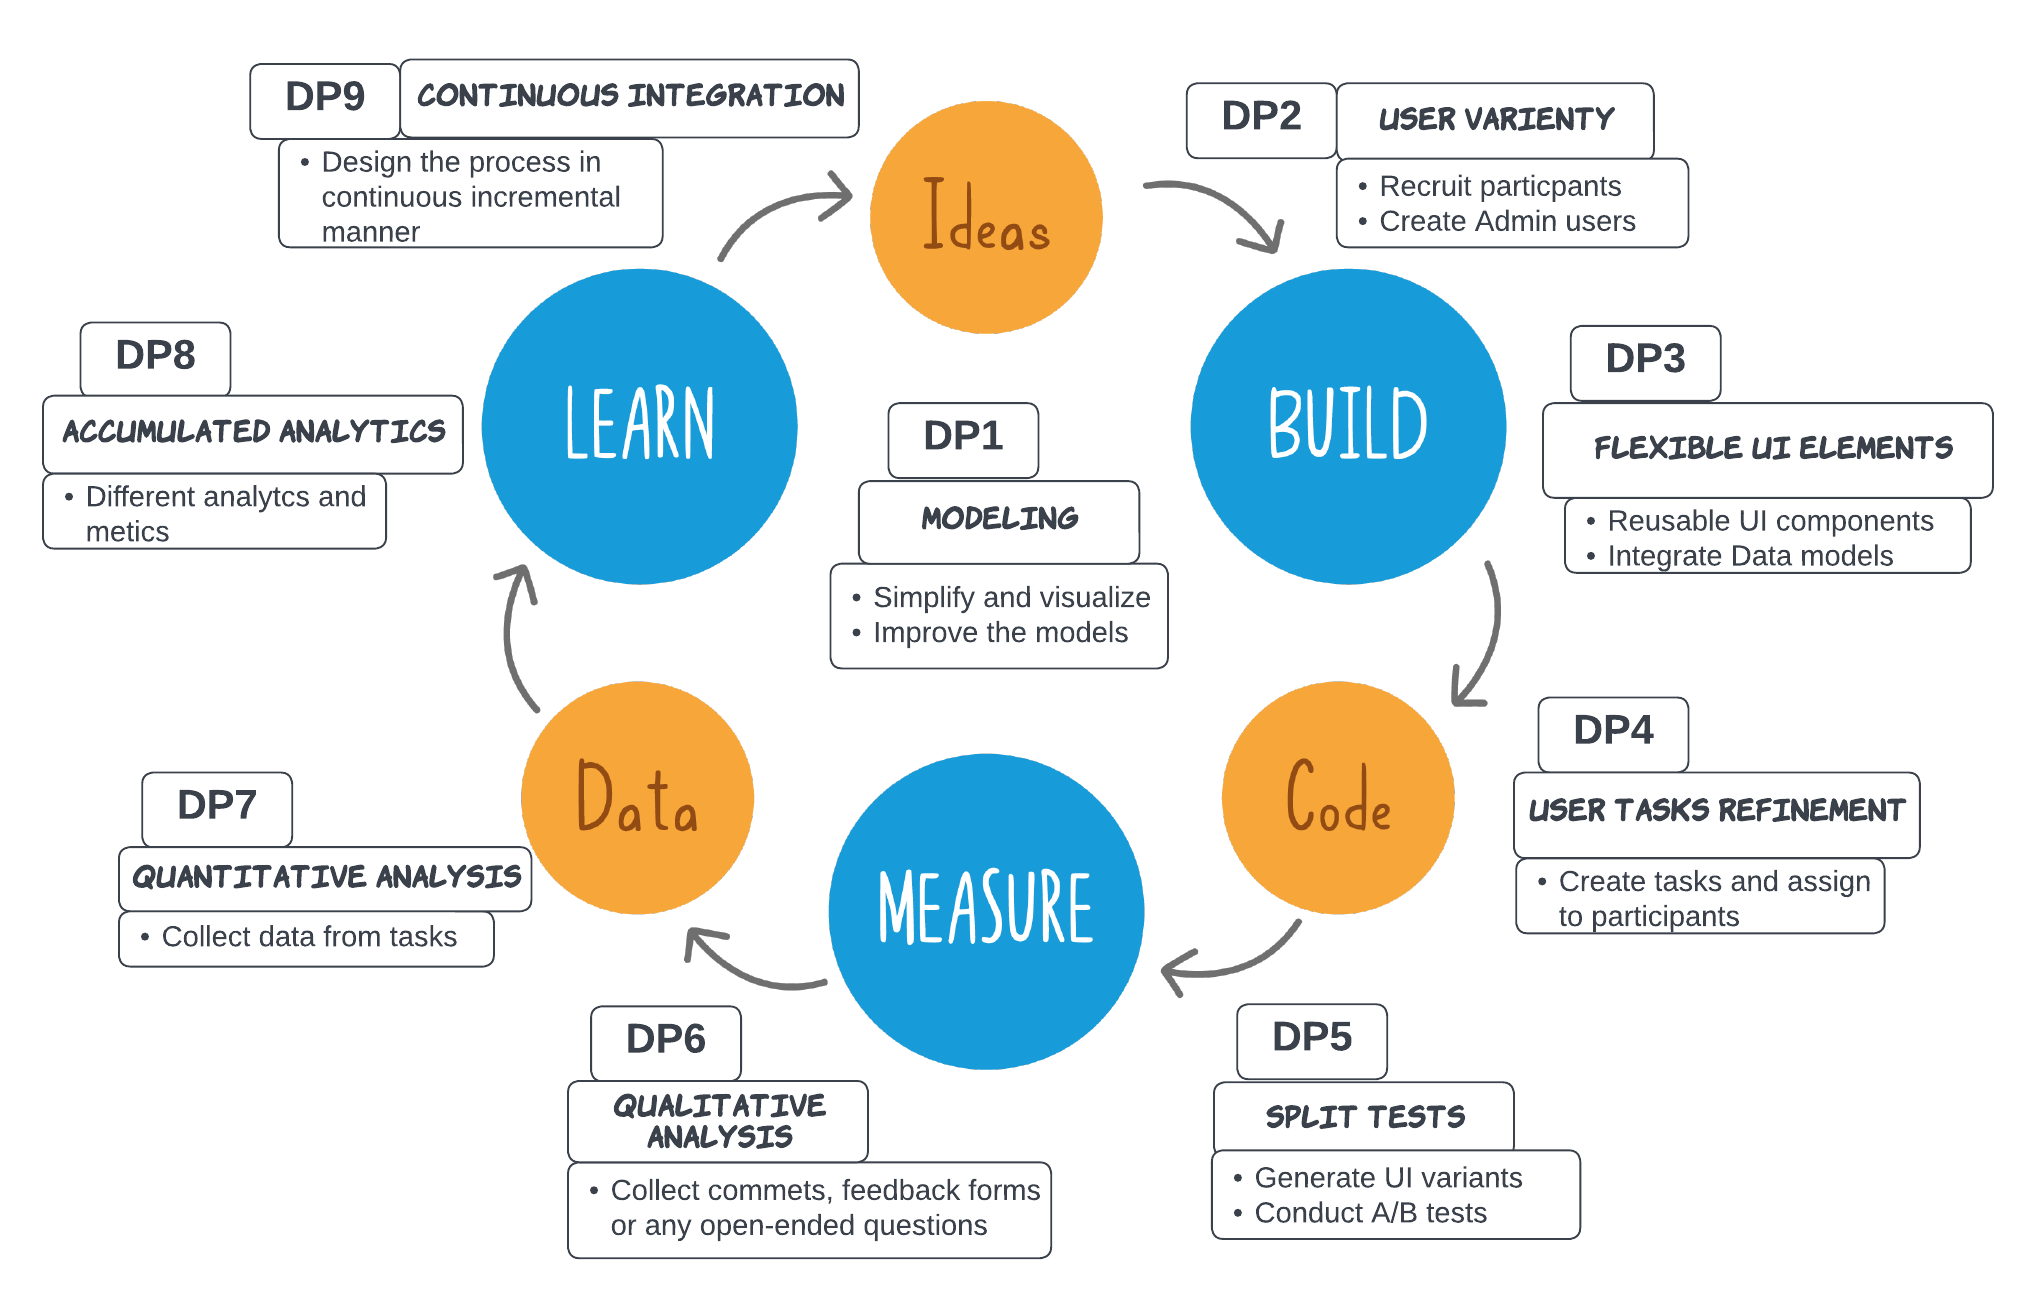
\includegraphics[width=0.8\textwidth]{LEAN-DPs.png}
  \caption[Solution Concept]{Overall Solution Design for a UI Prototyping tool using LEAN principles}
  \label{fig:design:lean}
\end{figure}

In the LEAN development cycle, the design of the whole process is done in a continuous iterative process (i.e., \ac{dp}3) for improvement of the solution approach.
%********************************** % Build **************************************** 
\paragraph{Build:}
\label{design:paragraph:build}
Initially, different stakeholders should be able to register to our tool (i.e., \ac{dp}1) having different rights. 
The tool administrators (i.e., the stakeholders) can build a UI prototype using various reusable UI components and create data models (i.e., \ac{dp}4). Using these UI elements and a drag-and-drop interface, we can make various screens and connect them to data models.
In the next step, we create various UI variants or versions for creating split tests (i.e., \ac{dp}2).
After creating split tests, users would create various tasks simulating real-world scenarios, assign them randomly to participants and collect feedback (i.e., \ac{dp}5).
%********************************** % Measure **************************************
\paragraph{Measure:}
\label{design:paragraph:measure}
In this phase, we measure the data we receive from the tasks by conducting qualitative (i.e., \ac{dp}6) and quantitative (i.e., \ac{dp}7) analysis.
The quantitative analysis is done from the data we collect from the tasks (e.g., the time taken, successfully finished tasks, etc.).
Similarly, the qualitative analysis is done by colleting the comments, open-ended questions etc. after the task is finished. 
%********************************** % Learn ****************************************
\paragraph{Learn:}
\label{design:paragraph:learn}
In this phase, the data received from the analysis is processed and visualized. 
The data is processed by aggregating and combining the results of the qualitative and the quantitative analysis (i.e., \ac{dp}8). 
Finally, the models are given feedback from the data analysis, improving the UI prototype and updating it with the winner variant (i.e., \ac{dp}9) as the default UI component.
The refined product can be deployed for the entire population (or all the users) using the deployment module of a no-code development platform.

\section{Summary}
\label{design:section:summary}
In summary, a well-written solution design chapter is essential to any project or product development process. 
It provides a clear and detailed roadmap for the development team to follow, ensuring that the end product meets the requirements and is designed using best practices and principles.